\documentclass[1p]{elsarticle_modified}
%\bibliographystyle{elsarticle-num}

%\usepackage[colorlinks]{hyperref}
%\usepackage{abbrmath_seonhwa} %\Abb, \Ascr, \Acal ,\Abf, \Afrak
\usepackage{amsfonts}
\usepackage{amssymb}
\usepackage{amsmath}
\usepackage{amsthm}
\usepackage{scalefnt}
\usepackage{amsbsy}
\usepackage{kotex}
\usepackage{caption}
\usepackage{subfig}
\usepackage{color}
\usepackage{graphicx}
\usepackage{xcolor} %% white, black, red, green, blue, cyan, magenta, yellow
\usepackage{float}
\usepackage{setspace}
\usepackage{hyperref}

\usepackage{tikz}
\usetikzlibrary{arrows}

\usepackage{multirow}
\usepackage{array} % fixed length table
\usepackage{hhline}

%%%%%%%%%%%%%%%%%%%%%
\makeatletter
\renewcommand*\env@matrix[1][\arraystretch]{%
	\edef\arraystretch{#1}%
	\hskip -\arraycolsep
	\let\@ifnextchar\new@ifnextchar
	\array{*\c@MaxMatrixCols c}}
\makeatother %https://tex.stackexchange.com/questions/14071/how-can-i-increase-the-line-spacing-in-a-matrix
%%%%%%%%%%%%%%%

\usepackage[normalem]{ulem}

\newcommand{\msout}[1]{\ifmmode\text{\sout{\ensuremath{#1}}}\else\sout{#1}\fi}
%SOURCE: \msout is \stkout macro in https://tex.stackexchange.com/questions/20609/strikeout-in-math-mode

\newcommand{\cancel}[1]{
	\ifmmode
	{\color{red}\msout{#1}}
	\else
	{\color{red}\sout{#1}}
	\fi
}

\newcommand{\add}[1]{
	{\color{blue}\uwave{#1}}
}

\newcommand{\replace}[2]{
	\ifmmode
	{\color{red}\msout{#1}}{\color{blue}\uwave{#2}}
	\else
	{\color{red}\sout{#1}}{\color{blue}\uwave{#2}}
	\fi
}

\newcommand{\Sol}{\mathcal{S}} %segment
\newcommand{\D}{D} %diagram
\newcommand{\A}{\mathcal{A}} %arc


%%%%%%%%%%%%%%%%%%%%%%%%%%%%%5 test

\def\sl{\operatorname{\textup{SL}}(2,\Cbb)}
\def\psl{\operatorname{\textup{PSL}}(2,\Cbb)}
\def\quan{\mkern 1mu \triangleright \mkern 1mu}

\theoremstyle{definition}
\newtheorem{thm}{Theorem}[section]
\newtheorem{prop}[thm]{Proposition}
\newtheorem{lem}[thm]{Lemma}
\newtheorem{ques}[thm]{Question}
\newtheorem{cor}[thm]{Corollary}
\newtheorem{defn}[thm]{Definition}
\newtheorem{exam}[thm]{Example}
\newtheorem{rmk}[thm]{Remark}
\newtheorem{alg}[thm]{Algorithm}

\newcommand{\I}{\sqrt{-1}}
\begin{document}

%\begin{frontmatter}
%
%\title{Boundary parabolic representations of knots up to 8 crossings}
%
%%% Group authors per affiliation:
%\author{Yunhi Cho} 
%\address{Department of Mathematics, University of Seoul, Seoul, Korea}
%\ead{yhcho@uos.ac.kr}
%
%
%\author{Seonhwa Kim} %\fnref{s_kim}}
%\address{Center for Geometry and Physics, Institute for Basic Science, Pohang, 37673, Korea}
%\ead{ryeona17@ibs.re.kr}
%
%\author{Hyuk Kim}
%\address{Department of Mathematical Sciences, Seoul National University, Seoul 08826, Korea}
%\ead{hyukkim@snu.ac.kr}
%
%\author{Seokbeom Yoon}
%\address{Department of Mathematical Sciences, Seoul National University, Seoul, 08826,  Korea}
%\ead{sbyoon15@snu.ac.kr}
%
%\begin{abstract}
%We find all boundary parabolic representation of knots up to 8 crossings.
%
%\end{abstract}
%\begin{keyword}
%    \MSC[2010] 57M25 
%\end{keyword}
%
%\end{frontmatter}

%\linenumbers
%\tableofcontents
%
\newcommand\colored[1]{\textcolor{white}{\rule[-0.35ex]{0.8em}{1.4ex}}\kern-0.8em\color{red} #1}%
%\newcommand\colored[1]{\textcolor{white}{ #1}\kern-2.17ex	\textcolor{white}{ #1}\kern-1.81ex	\textcolor{white}{ #1}\kern-2.15ex\color{red}#1	}

{\Large $\underline{12n_{0469}~(K12n_{0469})}$}

\setlength{\tabcolsep}{10pt}
\renewcommand{\arraystretch}{1.6}
\vspace{1cm}\begin{tabular}{m{100pt}>{\centering\arraybackslash}m{274pt}}
\multirow{5}{120pt}{
	\centering
	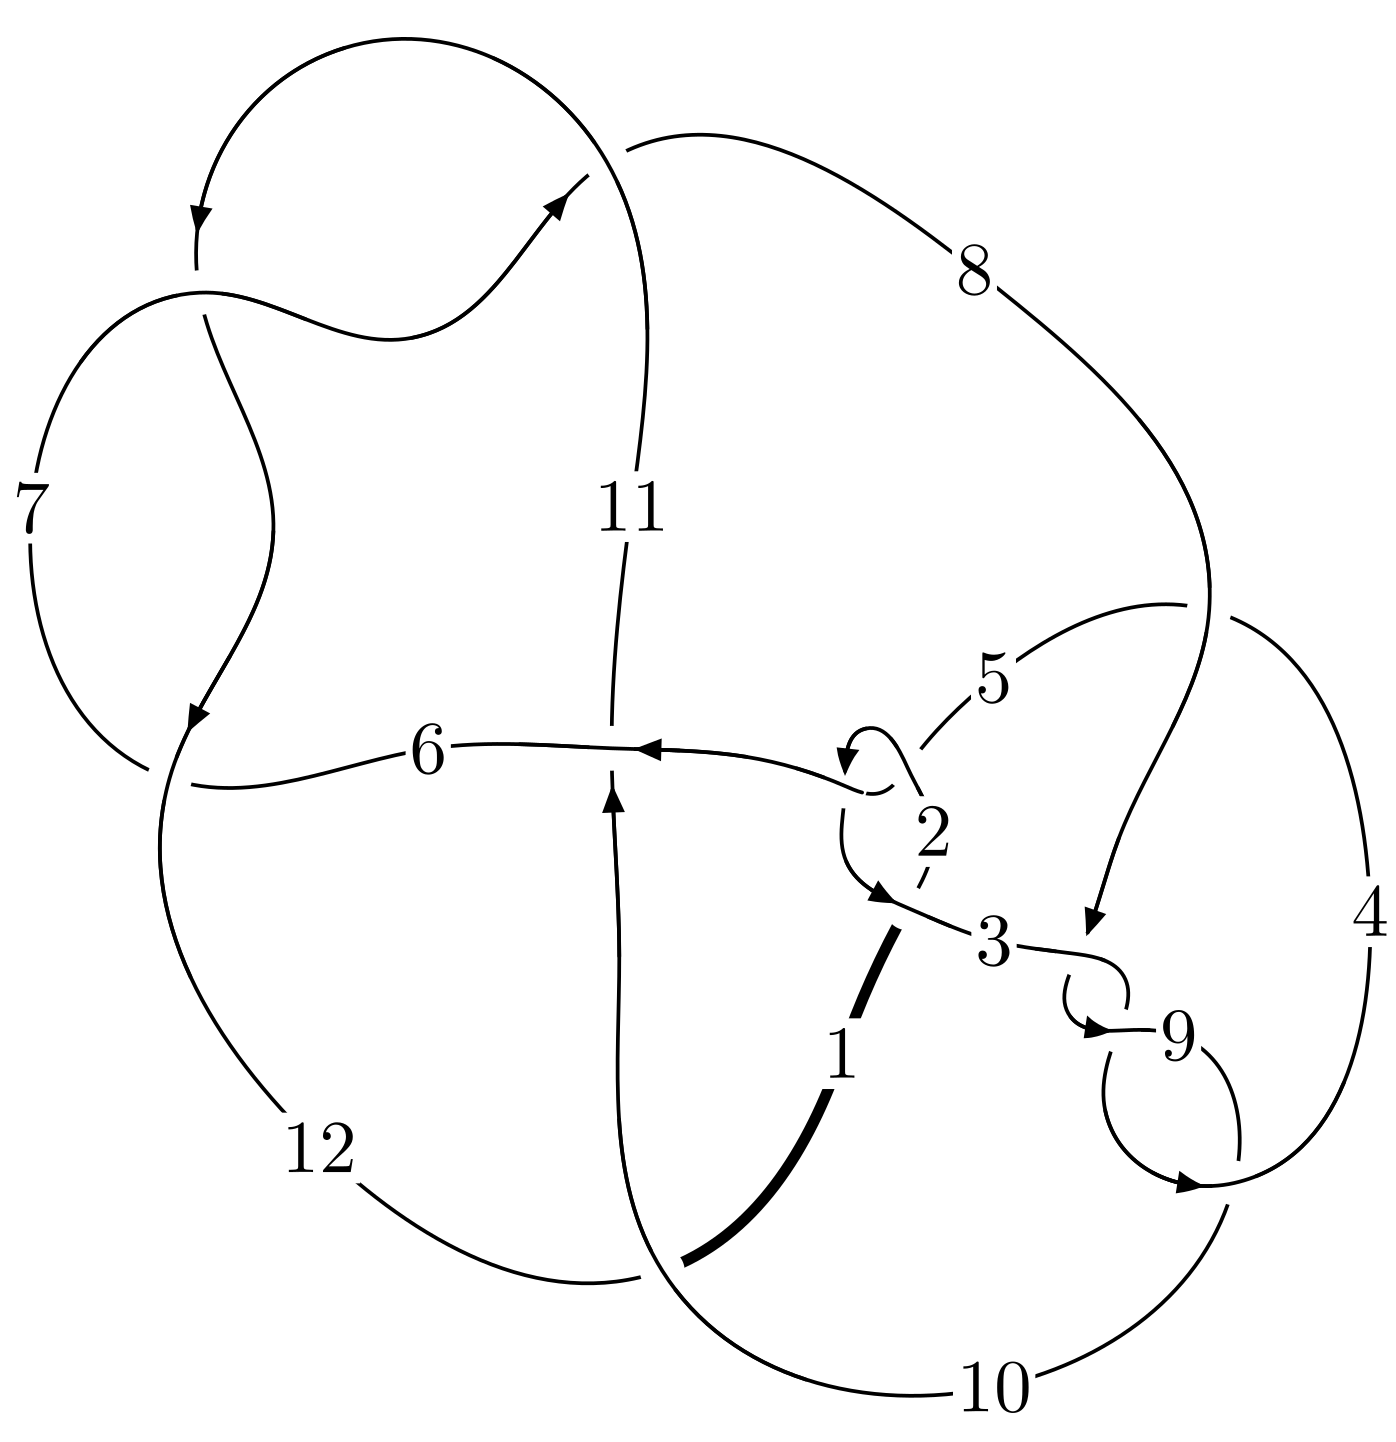
\includegraphics[width=112pt]{../../../GIT/diagram.site/Diagrams/png/2558_12n_0469.png}\\
\ \ \ A knot diagram\footnotemark}&
\allowdisplaybreaks
\textbf{Linearized knot diagam} \\
\cline{2-2}
 &
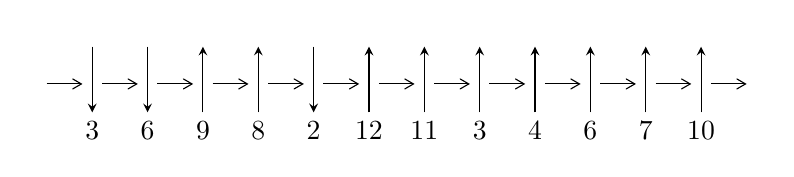
\begin{tikzpicture}[x=20pt, y=17pt]
	% nodes
	\node (C0) at (0, 0) {};
	\node (C1) at (1, 0) {};
	\node (C1U) at (1, +1) {};
	\node (C1D) at (1, -1) {3};

	\node (C2) at (2, 0) {};
	\node (C2U) at (2, +1) {};
	\node (C2D) at (2, -1) {6};

	\node (C3) at (3, 0) {};
	\node (C3U) at (3, +1) {};
	\node (C3D) at (3, -1) {9};

	\node (C4) at (4, 0) {};
	\node (C4U) at (4, +1) {};
	\node (C4D) at (4, -1) {8};

	\node (C5) at (5, 0) {};
	\node (C5U) at (5, +1) {};
	\node (C5D) at (5, -1) {2};

	\node (C6) at (6, 0) {};
	\node (C6U) at (6, +1) {};
	\node (C6D) at (6, -1) {12};

	\node (C7) at (7, 0) {};
	\node (C7U) at (7, +1) {};
	\node (C7D) at (7, -1) {11};

	\node (C8) at (8, 0) {};
	\node (C8U) at (8, +1) {};
	\node (C8D) at (8, -1) {3};

	\node (C9) at (9, 0) {};
	\node (C9U) at (9, +1) {};
	\node (C9D) at (9, -1) {4};

	\node (C10) at (10, 0) {};
	\node (C10U) at (10, +1) {};
	\node (C10D) at (10, -1) {6};

	\node (C11) at (11, 0) {};
	\node (C11U) at (11, +1) {};
	\node (C11D) at (11, -1) {7};

	\node (C12) at (12, 0) {};
	\node (C12U) at (12, +1) {};
	\node (C12D) at (12, -1) {10};
	\node (C13) at (13, 0) {};

	% arrows
	\draw[->,>={angle 60}]
	(C0) edge (C1) (C1) edge (C2) (C2) edge (C3) (C3) edge (C4) (C4) edge (C5) (C5) edge (C6) (C6) edge (C7) (C7) edge (C8) (C8) edge (C9) (C9) edge (C10) (C10) edge (C11) (C11) edge (C12) (C12) edge (C13) ;	\draw[->,>=stealth]
	(C1U) edge (C1D) (C2U) edge (C2D) (C3D) edge (C3U) (C4D) edge (C4U) (C5U) edge (C5D) (C6D) edge (C6U) (C7D) edge (C7U) (C8D) edge (C8U) (C9D) edge (C9U) (C10D) edge (C10U) (C11D) edge (C11U) (C12D) edge (C12U) ;
	\end{tikzpicture} \\
\hhline{~~} \\& 
\textbf{Solving Sequence} \\ \cline{2-2} 
 &
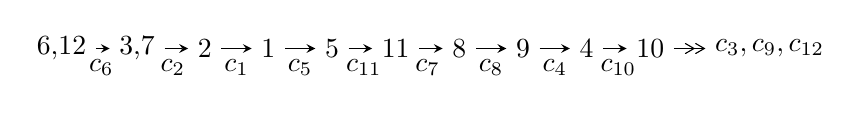
\begin{tikzpicture}[x=23pt, y=7pt]
	% node
	\node (A0) at (-1/8, 0) {6,12};
	\node (A1) at (17/16, 0) {3,7};
	\node (A2) at (17/8, 0) {2};
	\node (A3) at (25/8, 0) {1};
	\node (A4) at (33/8, 0) {5};
	\node (A5) at (41/8, 0) {11};
	\node (A6) at (49/8, 0) {8};
	\node (A7) at (57/8, 0) {9};
	\node (A8) at (65/8, 0) {4};
	\node (A9) at (73/8, 0) {10};
	\node (C1) at (1/2, -1) {$c_{6}$};
	\node (C2) at (13/8, -1) {$c_{2}$};
	\node (C3) at (21/8, -1) {$c_{1}$};
	\node (C4) at (29/8, -1) {$c_{5}$};
	\node (C5) at (37/8, -1) {$c_{11}$};
	\node (C6) at (45/8, -1) {$c_{7}$};
	\node (C7) at (53/8, -1) {$c_{8}$};
	\node (C8) at (61/8, -1) {$c_{4}$};
	\node (C9) at (69/8, -1) {$c_{10}$};
	\node (A10) at (11, 0) {$c_{3},c_{9},c_{12}$};

	% edge
	\draw[->,>=stealth]	
	(A0) edge (A1) (A1) edge (A2) (A2) edge (A3) (A3) edge (A4) (A4) edge (A5) (A5) edge (A6) (A6) edge (A7) (A7) edge (A8) (A8) edge (A9) ;
	\draw[->>,>={angle 60}]	
	(A9) edge (A10);
\end{tikzpicture} \\ 

\end{tabular} \\

\footnotetext{
The image of knot diagram is generated by the software ``\textbf{Draw programme}" developed by Andrew Bartholomew(\url{http://www.layer8.co.uk/maths/draw/index.htm\#Running-draw}), where we modified some parts for our purpose(\url{https://github.com/CATsTAILs/LinksPainter}).
}\phantom \\ \newline 
\centering \textbf{Ideals for irreducible components\footnotemark of $X_{\text{par}}$} 
 
\begin{align*}
I^u_{1}&=\langle 
271358647 u^{35}-529043524 u^{34}+\cdots+488920819 b-215606766,\\
\phantom{I^u_{1}}&\phantom{= \langle  }334439774 u^{35}-1269481739 u^{34}+\cdots+977841638 a-5972341699,\;u^{36}-2 u^{35}+\cdots-4 u-1\rangle \\
I^u_{2}&=\langle 
b+1,\;- u^2+a- u-2,\;u^3+u^2+2 u+1\rangle \\
I^u_{3}&=\langle 
b-1,\;2 u^2 a+a^2-2 a u+4 a+u-1,\;u^3- u^2+2 u-1\rangle \\
\\
\end{align*}
\raggedright * 3 irreducible components of $\dim_{\mathbb{C}}=0$, with total 45 representations.\\
\footnotetext{All coefficients of polynomials are rational numbers. But the coefficients are sometimes approximated in decimal forms when there is not enough margin.}
\newpage
\renewcommand{\arraystretch}{1}
\centering \section*{I. $I^u_{1}= \langle 2.71\times10^{8} u^{35}-5.29\times10^{8} u^{34}+\cdots+4.89\times10^{8} b-2.16\times10^{8},\;3.34\times10^{8} u^{35}-1.27\times10^{9} u^{34}+\cdots+9.78\times10^{8} a-5.97\times10^{9},\;u^{36}-2 u^{35}+\cdots-4 u-1 \rangle$}
\flushleft \textbf{(i) Arc colorings}\\
\begin{tabular}{m{7pt} m{180pt} m{7pt} m{180pt} }
\flushright $a_{6}=$&$\begin{pmatrix}1\\0\end{pmatrix}$ \\
\flushright $a_{12}=$&$\begin{pmatrix}0\\u\end{pmatrix}$ \\
\flushright $a_{3}=$&$\begin{pmatrix}-0.342018 u^{35}+1.29825 u^{34}+\cdots-14.1375 u+6.10768\\-0.555016 u^{35}+1.08206 u^{34}+\cdots-2.96956 u+0.440985\end{pmatrix}$ \\
\flushright $a_{7}=$&$\begin{pmatrix}1\\- u^2\end{pmatrix}$ \\
\flushright $a_{2}=$&$\begin{pmatrix}-0.897034 u^{35}+2.38031 u^{34}+\cdots-17.1071 u+6.54866\\-0.555016 u^{35}+1.08206 u^{34}+\cdots-2.96956 u+0.440985\end{pmatrix}$ \\
\flushright $a_{1}=$&$\begin{pmatrix}u^7+4 u^5+4 u^3\\- u^7-3 u^5-2 u^3+u\end{pmatrix}$ \\
\flushright $a_{5}=$&$\begin{pmatrix}1.04147 u^{35}-2.64685 u^{34}+\cdots+19.6688 u-5.62579\\0.678551 u^{35}-1.22102 u^{34}+\cdots+3.80116 u-0.427325\end{pmatrix}$ \\
\flushright $a_{11}=$&$\begin{pmatrix}- u\\u^3+u\end{pmatrix}$ \\
\flushright $a_{8}=$&$\begin{pmatrix}u^2+1\\- u^4-2 u^2\end{pmatrix}$ \\
\flushright $a_{9}=$&$\begin{pmatrix}1.07868 u^{35}-2.14851 u^{34}+\cdots+24.9712 u-6.81062\\-0.00885463 u^{35}-0.0464490 u^{34}+\cdots+2.49588 u-1.07868\end{pmatrix}$ \\
\flushright $a_{4}=$&$\begin{pmatrix}0.440985 u^{35}-1.43699 u^{34}+\cdots+15.6653 u-4.73350\\0.614212 u^{35}-1.25941 u^{34}+\cdots+4.73960 u-0.342018\end{pmatrix}$ \\
\flushright $a_{10}=$&$\begin{pmatrix}- u^3-2 u\\u^3+u\end{pmatrix}$\\&\end{tabular}
\flushleft \textbf{(ii) Obstruction class $= -1$}\\~\\
\flushleft \textbf{(iii) Cusp Shapes $= \frac{259508424}{488920819} u^{35}-\frac{190324579}{488920819} u^{34}+\cdots+\frac{7239334870}{488920819} u+\frac{1820082994}{488920819}$}\\~\\
\newpage\renewcommand{\arraystretch}{1}
\flushleft \textbf{(iv) u-Polynomials at the component}\newline \\
\begin{tabular}{m{50pt}|m{274pt}}
Crossings & \hspace{64pt}u-Polynomials at each crossing \\
\hline $$\begin{aligned}c_{1}\end{aligned}$$&$\begin{aligned}
&u^{36}+46 u^{35}+\cdots+1827 u+49
\end{aligned}$\\
\hline $$\begin{aligned}c_{2},c_{5}\end{aligned}$$&$\begin{aligned}
&u^{36}+4 u^{35}+\cdots+91 u-7
\end{aligned}$\\
\hline $$\begin{aligned}c_{3},c_{8},c_{9}\end{aligned}$$&$\begin{aligned}
&u^{36}+u^{35}+\cdots-8 u-8
\end{aligned}$\\
\hline $$\begin{aligned}c_{4}\end{aligned}$$&$\begin{aligned}
&u^{36}-3 u^{35}+\cdots+8 u-8
\end{aligned}$\\
\hline $$\begin{aligned}c_{6},c_{7},c_{11}\end{aligned}$$&$\begin{aligned}
&u^{36}-2 u^{35}+\cdots-4 u-1
\end{aligned}$\\
\hline $$\begin{aligned}c_{10}\end{aligned}$$&$\begin{aligned}
&u^{36}+2 u^{35}+\cdots-2232 u-481
\end{aligned}$\\
\hline $$\begin{aligned}c_{12}\end{aligned}$$&$\begin{aligned}
&u^{36}+4 u^{35}+\cdots-16 u+1
\end{aligned}$\\
\hline
\end{tabular}\\~\\
\newpage\renewcommand{\arraystretch}{1}
\flushleft \textbf{(v) Riley Polynomials at the component}\newline \\
\begin{tabular}{m{50pt}|m{274pt}}
Crossings & \hspace{64pt}Riley Polynomials at each crossing \\
\hline $$\begin{aligned}c_{1}\end{aligned}$$&$\begin{aligned}
&y^{36}-102 y^{35}+\cdots-1510327 y+2401
\end{aligned}$\\
\hline $$\begin{aligned}c_{2},c_{5}\end{aligned}$$&$\begin{aligned}
&y^{36}-46 y^{35}+\cdots-1827 y+49
\end{aligned}$\\
\hline $$\begin{aligned}c_{3},c_{8},c_{9}\end{aligned}$$&$\begin{aligned}
&y^{36}-29 y^{35}+\cdots-832 y+64
\end{aligned}$\\
\hline $$\begin{aligned}c_{4}\end{aligned}$$&$\begin{aligned}
&y^{36}+55 y^{35}+\cdots-1728 y+64
\end{aligned}$\\
\hline $$\begin{aligned}c_{6},c_{7},c_{11}\end{aligned}$$&$\begin{aligned}
&y^{36}+36 y^{35}+\cdots-52 y+1
\end{aligned}$\\
\hline $$\begin{aligned}c_{10}\end{aligned}$$&$\begin{aligned}
&y^{36}+20 y^{35}+\cdots-9532084 y+231361
\end{aligned}$\\
\hline $$\begin{aligned}c_{12}\end{aligned}$$&$\begin{aligned}
&y^{36}+44 y^{35}+\cdots-532 y+1
\end{aligned}$\\
\hline
\end{tabular}\\~\\
\newpage\flushleft \textbf{(vi) Complex Volumes and Cusp Shapes}
$$\begin{array}{c|c|c}  
\text{Solutions to }I^u_{1}& \I (\text{vol} + \sqrt{-1}CS) & \text{Cusp shape}\\
 \hline 
\begin{aligned}
u &= -0.746590 + 0.534072 I \\
a &= -1.14025 - 1.14185 I \\
b &= \phantom{-}1.71941 + 0.06440 I\end{aligned}
 & -10.55280 - 2.49065 I & \phantom{-}2.28481 + 2.78156 I \\ \hline\begin{aligned}
u &= -0.746590 - 0.534072 I \\
a &= -1.14025 + 1.14185 I \\
b &= \phantom{-}1.71941 - 0.06440 I\end{aligned}
 & -10.55280 + 2.49065 I & \phantom{-}2.28481 - 2.78156 I \\ \hline\begin{aligned}
u &= \phantom{-}0.664083 + 0.631741 I \\
a &= \phantom{-}1.014470 - 0.540455 I \\
b &= -1.67188 - 0.14945 I\end{aligned}
 & -6.71821 - 3.14670 I & \phantom{-}4.48459 + 0.40539 I \\ \hline\begin{aligned}
u &= \phantom{-}0.664083 - 0.631741 I \\
a &= \phantom{-}1.014470 + 0.540455 I \\
b &= -1.67188 + 0.14945 I\end{aligned}
 & -6.71821 + 3.14670 I & \phantom{-}4.48459 - 0.40539 I \\ \hline\begin{aligned}
u &= \phantom{-}0.784223 + 0.433590 I \\
a &= \phantom{-}1.14935 - 1.67783 I \\
b &= -1.65415 + 0.25580 I\end{aligned}
 & -6.05301 + 8.02106 I & \phantom{-}5.69652 - 5.48227 I \\ \hline\begin{aligned}
u &= \phantom{-}0.784223 - 0.433590 I \\
a &= \phantom{-}1.14935 + 1.67783 I \\
b &= -1.65415 - 0.25580 I\end{aligned}
 & -6.05301 - 8.02106 I & \phantom{-}5.69652 + 5.48227 I \\ \hline\begin{aligned}
u &= -0.754684\phantom{ +0.000000I} \\
a &= \phantom{-}2.04702\phantom{ +0.000000I} \\
b &= -1.31973\phantom{ +0.000000I}\end{aligned}
 & \phantom{-}0.746951\phantom{ +0.000000I} & \phantom{-}8.79890\phantom{ +0.000000I} \\ \hline\begin{aligned}
u &= -0.202995 + 1.255340 I \\
a &= -0.951854 - 0.726217 I \\
b &= \phantom{-}0.175613 + 0.296050 I\end{aligned}
 & \phantom{-}2.08619 - 3.03413 I & \phantom{-}10.51311 + 3.79199 I \\ \hline\begin{aligned}
u &= -0.202995 - 1.255340 I \\
a &= -0.951854 + 0.726217 I \\
b &= \phantom{-}0.175613 - 0.296050 I\end{aligned}
 & \phantom{-}2.08619 + 3.03413 I & \phantom{-}10.51311 - 3.79199 I \\ \hline\begin{aligned}
u &= \phantom{-}0.597158 + 0.410952 I \\
a &= -0.03383 + 1.92390 I \\
b &= \phantom{-}0.617286 - 0.749282 I\end{aligned}
 & \phantom{-}1.66187 + 4.15562 I & \phantom{-}8.00287 - 6.91393 I\\
 \hline 
 \end{array}$$\newpage$$\begin{array}{c|c|c}  
\text{Solutions to }I^u_{1}& \I (\text{vol} + \sqrt{-1}CS) & \text{Cusp shape}\\
 \hline 
\begin{aligned}
u &= \phantom{-}0.597158 - 0.410952 I \\
a &= -0.03383 - 1.92390 I \\
b &= \phantom{-}0.617286 + 0.749282 I\end{aligned}
 & \phantom{-}1.66187 - 4.15562 I & \phantom{-}8.00287 + 6.91393 I \\ \hline\begin{aligned}
u &= -0.326127 + 1.248070 I \\
a &= \phantom{-}0.633554 + 0.938984 I \\
b &= -1.359350 + 0.009058 I\end{aligned}
 & -3.12452 - 3.89594 I & \phantom{-}3.97835 + 4.14640 I \\ \hline\begin{aligned}
u &= -0.326127 - 1.248070 I \\
a &= \phantom{-}0.633554 - 0.938984 I \\
b &= -1.359350 - 0.009058 I\end{aligned}
 & -3.12452 + 3.89594 I & \phantom{-}3.97835 - 4.14640 I \\ \hline\begin{aligned}
u &= \phantom{-}0.504679 + 0.396227 I \\
a &= -1.116890 - 0.669513 I \\
b &= \phantom{-}0.659666 + 0.583318 I\end{aligned}
 & \phantom{-}1.51779 - 0.52826 I & \phantom{-}7.65473 - 0.24051 I \\ \hline\begin{aligned}
u &= \phantom{-}0.504679 - 0.396227 I \\
a &= -1.116890 + 0.669513 I \\
b &= \phantom{-}0.659666 - 0.583318 I\end{aligned}
 & \phantom{-}1.51779 + 0.52826 I & \phantom{-}7.65473 + 0.24051 I \\ \hline\begin{aligned}
u &= -0.631586\phantom{ +0.000000I} \\
a &= -1.76477\phantom{ +0.000000I} \\
b &= \phantom{-}0.225322\phantom{ +0.000000I}\end{aligned}
 & \phantom{-}5.91452\phantom{ +0.000000I} & \phantom{-}16.7470\phantom{ +0.000000I} \\ \hline\begin{aligned}
u &= \phantom{-}0.096853 + 1.373970 I \\
a &= \phantom{-}0.057014 - 0.382407 I \\
b &= \phantom{-}0.233991 + 0.646152 I\end{aligned}
 & -3.76081 + 1.82148 I & \phantom{-}4.18456 - 2.97690 I \\ \hline\begin{aligned}
u &= \phantom{-}0.096853 - 1.373970 I \\
a &= \phantom{-}0.057014 + 0.382407 I \\
b &= \phantom{-}0.233991 - 0.646152 I\end{aligned}
 & -3.76081 - 1.82148 I & \phantom{-}4.18456 + 2.97690 I \\ \hline\begin{aligned}
u &= -0.032206 + 1.383860 I \\
a &= \phantom{-}0.93309 + 1.09446 I \\
b &= \phantom{-}1.227970 - 0.334502 I\end{aligned}
 & -1.31636 - 0.59124 I & \phantom{-}2.44003 + 0. I\phantom{ +0.000000I} \\ \hline\begin{aligned}
u &= -0.032206 - 1.383860 I \\
a &= \phantom{-}0.93309 - 1.09446 I \\
b &= \phantom{-}1.227970 + 0.334502 I\end{aligned}
 & -1.31636 + 0.59124 I & \phantom{-}2.44003 + 0. I\phantom{ +0.000000I}\\
 \hline 
 \end{array}$$\newpage$$\begin{array}{c|c|c}  
\text{Solutions to }I^u_{1}& \I (\text{vol} + \sqrt{-1}CS) & \text{Cusp shape}\\
 \hline 
\begin{aligned}
u &= \phantom{-}0.209916 + 1.383740 I \\
a &= -0.161570 + 0.134658 I \\
b &= \phantom{-}0.763567 + 0.425752 I\end{aligned}
 & -4.01585 + 2.05418 I & \phantom{-}4.74740 + 1.07135 I \\ \hline\begin{aligned}
u &= \phantom{-}0.209916 - 1.383740 I \\
a &= -0.161570 - 0.134658 I \\
b &= \phantom{-}0.763567 - 0.425752 I\end{aligned}
 & -4.01585 - 2.05418 I & \phantom{-}4.74740 - 1.07135 I \\ \hline\begin{aligned}
u &= -0.10642 + 1.44688 I \\
a &= -0.474212 + 0.967148 I \\
b &= -1.044990 - 0.635725 I\end{aligned}
 & -7.20243 - 2.62870 I & \phantom{-0.000000 -}0. + 1.56071 I \\ \hline\begin{aligned}
u &= -0.10642 - 1.44688 I \\
a &= -0.474212 - 0.967148 I \\
b &= -1.044990 + 0.635725 I\end{aligned}
 & -7.20243 + 2.62870 I & \phantom{-0.000000 } 0. - 1.56071 I \\ \hline\begin{aligned}
u &= \phantom{-}0.21082 + 1.46540 I \\
a &= \phantom{-}0.586263 + 1.079000 I \\
b &= \phantom{-}0.693691 - 0.900679 I\end{aligned}
 & -4.41494 + 7.10948 I & \phantom{-}6.00000 - 5.97206 I \\ \hline\begin{aligned}
u &= \phantom{-}0.21082 - 1.46540 I \\
a &= \phantom{-}0.586263 - 1.079000 I \\
b &= \phantom{-}0.693691 + 0.900679 I\end{aligned}
 & -4.41494 - 7.10948 I & \phantom{-}6.00000 + 5.97206 I \\ \hline\begin{aligned}
u &= \phantom{-}0.29360 + 1.49537 I \\
a &= -0.31496 - 1.59906 I \\
b &= -1.68265 + 0.33795 I\end{aligned}
 & -12.2864 + 11.9589 I & \phantom{-0.000000 } 0 \\ \hline\begin{aligned}
u &= \phantom{-}0.29360 - 1.49537 I \\
a &= -0.31496 + 1.59906 I \\
b &= -1.68265 - 0.33795 I\end{aligned}
 & -12.2864 - 11.9589 I & \phantom{-0.000000 } 0 \\ \hline\begin{aligned}
u &= -0.334693 + 0.338551 I \\
a &= \phantom{-}0.58755 + 1.75938 I \\
b &= -0.790374 - 0.317839 I\end{aligned}
 & -1.37785 - 1.03574 I & -0.30331 + 3.73142 I \\ \hline\begin{aligned}
u &= -0.334693 - 0.338551 I \\
a &= \phantom{-}0.58755 - 1.75938 I \\
b &= -0.790374 + 0.317839 I\end{aligned}
 & -1.37785 + 1.03574 I & -0.30331 - 3.73142 I\\
 \hline 
 \end{array}$$\newpage$$\begin{array}{c|c|c}  
\text{Solutions to }I^u_{1}& \I (\text{vol} + \sqrt{-1}CS) & \text{Cusp shape}\\
 \hline 
\begin{aligned}
u &= -0.25500 + 1.53176 I \\
a &= \phantom{-}0.269560 - 1.152100 I \\
b &= \phantom{-}1.79484 + 0.16936 I\end{aligned}
 & -17.3048 - 6.1571 I & \phantom{-0.000000 } 0 \\ \hline\begin{aligned}
u &= -0.25500 - 1.53176 I \\
a &= \phantom{-}0.269560 + 1.152100 I \\
b &= \phantom{-}1.79484 - 0.16936 I\end{aligned}
 & -17.3048 + 6.1571 I & \phantom{-0.000000 } 0 \\ \hline\begin{aligned}
u &= \phantom{-}0.19273 + 1.54392 I \\
a &= -0.368636 - 0.625846 I \\
b &= -1.78522 - 0.06510 I\end{aligned}
 & -13.90280 - 0.08031 I & \phantom{-0.000000 } 0 \\ \hline\begin{aligned}
u &= \phantom{-}0.19273 - 1.54392 I \\
a &= -0.368636 + 0.625846 I \\
b &= -1.78522 + 0.06510 I\end{aligned}
 & -13.90280 + 0.08031 I & \phantom{-0.000000 } 0 \\ \hline\begin{aligned}
u &= \phantom{-}0.431723\phantom{ +0.000000I} \\
a &= \phantom{-}0.157248\phantom{ +0.000000I} \\
b &= \phantom{-}0.236175\phantom{ +0.000000I}\end{aligned}
 & \phantom{-}0.680363\phantom{ +0.000000I} & \phantom{-}15.1480\phantom{ +0.000000I} \\ \hline\begin{aligned}
u &= -0.145505\phantom{ +0.000000I} \\
a &= \phantom{-}8.22319\phantom{ +0.000000I} \\
b &= \phantom{-}1.06341\phantom{ +0.000000I}\end{aligned}
 & \phantom{-}3.33955\phantom{ +0.000000I} & \phantom{-}1.75020\phantom{ +0.000000I}\\
 \hline 
 \end{array}$$\newpage\newpage\renewcommand{\arraystretch}{1}
\centering \section*{II. $I^u_{2}= \langle b+1,\;- u^2+a- u-2,\;u^3+u^2+2 u+1 \rangle$}
\flushleft \textbf{(i) Arc colorings}\\
\begin{tabular}{m{7pt} m{180pt} m{7pt} m{180pt} }
\flushright $a_{6}=$&$\begin{pmatrix}1\\0\end{pmatrix}$ \\
\flushright $a_{12}=$&$\begin{pmatrix}0\\u\end{pmatrix}$ \\
\flushright $a_{3}=$&$\begin{pmatrix}u^2+u+2\\-1\end{pmatrix}$ \\
\flushright $a_{7}=$&$\begin{pmatrix}1\\- u^2\end{pmatrix}$ \\
\flushright $a_{2}=$&$\begin{pmatrix}u^2+u+1\\-1\end{pmatrix}$ \\
\flushright $a_{1}=$&$\begin{pmatrix}-1\\0\end{pmatrix}$ \\
\flushright $a_{5}=$&$\begin{pmatrix}u^2+u+2\\-1\end{pmatrix}$ \\
\flushright $a_{11}=$&$\begin{pmatrix}- u\\- u^2- u-1\end{pmatrix}$ \\
\flushright $a_{8}=$&$\begin{pmatrix}u^2+1\\- u^2- u-1\end{pmatrix}$ \\
\flushright $a_{9}=$&$\begin{pmatrix}u^2+1\\- u^2- u-1\end{pmatrix}$ \\
\flushright $a_{4}=$&$\begin{pmatrix}u^2+u+2\\-1\end{pmatrix}$ \\
\flushright $a_{10}=$&$\begin{pmatrix}u^2+1\\- u^2- u-1\end{pmatrix}$\\&\end{tabular}
\flushleft \textbf{(ii) Obstruction class $= 1$}\\~\\
\flushleft \textbf{(iii) Cusp Shapes $= 2 u^2+4 u+4$}\\~\\
\newpage\renewcommand{\arraystretch}{1}
\flushleft \textbf{(iv) u-Polynomials at the component}\newline \\
\begin{tabular}{m{50pt}|m{274pt}}
Crossings & \hspace{64pt}u-Polynomials at each crossing \\
\hline $$\begin{aligned}c_{1},c_{2}\end{aligned}$$&$\begin{aligned}
&(u-1)^3
\end{aligned}$\\
\hline $$\begin{aligned}c_{3},c_{4},c_{8}\\c_{9}\end{aligned}$$&$\begin{aligned}
&u^3
\end{aligned}$\\
\hline $$\begin{aligned}c_{5}\end{aligned}$$&$\begin{aligned}
&(u+1)^3
\end{aligned}$\\
\hline $$\begin{aligned}c_{6},c_{7}\end{aligned}$$&$\begin{aligned}
&u^3+u^2+2 u+1
\end{aligned}$\\
\hline $$\begin{aligned}c_{10},c_{12}\end{aligned}$$&$\begin{aligned}
&u^3+u^2-1
\end{aligned}$\\
\hline $$\begin{aligned}c_{11}\end{aligned}$$&$\begin{aligned}
&u^3- u^2+2 u-1
\end{aligned}$\\
\hline
\end{tabular}\\~\\
\newpage\renewcommand{\arraystretch}{1}
\flushleft \textbf{(v) Riley Polynomials at the component}\newline \\
\begin{tabular}{m{50pt}|m{274pt}}
Crossings & \hspace{64pt}Riley Polynomials at each crossing \\
\hline $$\begin{aligned}c_{1},c_{2},c_{5}\end{aligned}$$&$\begin{aligned}
&(y-1)^3
\end{aligned}$\\
\hline $$\begin{aligned}c_{3},c_{4},c_{8}\\c_{9}\end{aligned}$$&$\begin{aligned}
&y^3
\end{aligned}$\\
\hline $$\begin{aligned}c_{6},c_{7},c_{11}\end{aligned}$$&$\begin{aligned}
&y^3+3 y^2+2 y-1
\end{aligned}$\\
\hline $$\begin{aligned}c_{10},c_{12}\end{aligned}$$&$\begin{aligned}
&y^3- y^2+2 y-1
\end{aligned}$\\
\hline
\end{tabular}\\~\\
\newpage\flushleft \textbf{(vi) Complex Volumes and Cusp Shapes}
$$\begin{array}{c|c|c}  
\text{Solutions to }I^u_{2}& \I (\text{vol} + \sqrt{-1}CS) & \text{Cusp shape}\\
 \hline 
\begin{aligned}
u &= -0.215080 + 1.307140 I \\
a &= \phantom{-}0.122561 + 0.744862 I \\
b &= -1.00000\phantom{ +0.000000I}\end{aligned}
 & -4.66906 - 2.82812 I & -0.18504 + 4.10401 I \\ \hline\begin{aligned}
u &= -0.215080 - 1.307140 I \\
a &= \phantom{-}0.122561 - 0.744862 I \\
b &= -1.00000\phantom{ +0.000000I}\end{aligned}
 & -4.66906 + 2.82812 I & -0.18504 - 4.10401 I \\ \hline\begin{aligned}
u &= -0.569840\phantom{ +0.000000I} \\
a &= \phantom{-}1.75488\phantom{ +0.000000I} \\
b &= -1.00000\phantom{ +0.000000I}\end{aligned}
 & -0.531480\phantom{ +0.000000I} & \phantom{-}2.37010\phantom{ +0.000000I}\\
 \hline 
 \end{array}$$\newpage\newpage\renewcommand{\arraystretch}{1}
\centering \section*{III. $I^u_{3}= \langle b-1,\;2 u^2 a+a^2-2 a u+4 a+u-1,\;u^3- u^2+2 u-1 \rangle$}
\flushleft \textbf{(i) Arc colorings}\\
\begin{tabular}{m{7pt} m{180pt} m{7pt} m{180pt} }
\flushright $a_{6}=$&$\begin{pmatrix}1\\0\end{pmatrix}$ \\
\flushright $a_{12}=$&$\begin{pmatrix}0\\u\end{pmatrix}$ \\
\flushright $a_{3}=$&$\begin{pmatrix}a\\1\end{pmatrix}$ \\
\flushright $a_{7}=$&$\begin{pmatrix}1\\- u^2\end{pmatrix}$ \\
\flushright $a_{2}=$&$\begin{pmatrix}a+1\\1\end{pmatrix}$ \\
\flushright $a_{1}=$&$\begin{pmatrix}1\\0\end{pmatrix}$ \\
\flushright $a_{5}=$&$\begin{pmatrix}- a\\-1\end{pmatrix}$ \\
\flushright $a_{11}=$&$\begin{pmatrix}- u\\u^2- u+1\end{pmatrix}$ \\
\flushright $a_{8}=$&$\begin{pmatrix}u^2+1\\- u^2+u-1\end{pmatrix}$ \\
\flushright $a_{9}=$&$\begin{pmatrix}u^2 a+a+1\\- u^2 a+a u-2 u^2- a+u-2\end{pmatrix}$ \\
\flushright $a_{4}=$&$\begin{pmatrix}u^2- u+2\\- a u-2\end{pmatrix}$ \\
\flushright $a_{10}=$&$\begin{pmatrix}- u^2-1\\u^2- u+1\end{pmatrix}$\\&\end{tabular}
\flushleft \textbf{(ii) Obstruction class $= 1$}\\~\\
\flushleft \textbf{(iii) Cusp Shapes $= 4 u^2-4 u+12$}\\~\\
\newpage\renewcommand{\arraystretch}{1}
\flushleft \textbf{(iv) u-Polynomials at the component}\newline \\
\begin{tabular}{m{50pt}|m{274pt}}
Crossings & \hspace{64pt}u-Polynomials at each crossing \\
\hline $$\begin{aligned}c_{1},c_{5}\end{aligned}$$&$\begin{aligned}
&(u-1)^6
\end{aligned}$\\
\hline $$\begin{aligned}c_{2}\end{aligned}$$&$\begin{aligned}
&(u+1)^6
\end{aligned}$\\
\hline $$\begin{aligned}c_{3},c_{4},c_{8}\\c_{9}\end{aligned}$$&$\begin{aligned}
&(u^2-2)^3
\end{aligned}$\\
\hline $$\begin{aligned}c_{6},c_{7}\end{aligned}$$&$\begin{aligned}
&(u^3- u^2+2 u-1)^2
\end{aligned}$\\
\hline $$\begin{aligned}c_{10}\end{aligned}$$&$\begin{aligned}
&(u^3- u^2+1)^2
\end{aligned}$\\
\hline $$\begin{aligned}c_{11}\end{aligned}$$&$\begin{aligned}
&(u^3+u^2+2 u+1)^2
\end{aligned}$\\
\hline $$\begin{aligned}c_{12}\end{aligned}$$&$\begin{aligned}
&(u^3+u^2-1)^2
\end{aligned}$\\
\hline
\end{tabular}\\~\\
\newpage\renewcommand{\arraystretch}{1}
\flushleft \textbf{(v) Riley Polynomials at the component}\newline \\
\begin{tabular}{m{50pt}|m{274pt}}
Crossings & \hspace{64pt}Riley Polynomials at each crossing \\
\hline $$\begin{aligned}c_{1},c_{2},c_{5}\end{aligned}$$&$\begin{aligned}
&(y-1)^6
\end{aligned}$\\
\hline $$\begin{aligned}c_{3},c_{4},c_{8}\\c_{9}\end{aligned}$$&$\begin{aligned}
&(y-2)^6
\end{aligned}$\\
\hline $$\begin{aligned}c_{6},c_{7},c_{11}\end{aligned}$$&$\begin{aligned}
&(y^3+3 y^2+2 y-1)^2
\end{aligned}$\\
\hline $$\begin{aligned}c_{10},c_{12}\end{aligned}$$&$\begin{aligned}
&(y^3- y^2+2 y-1)^2
\end{aligned}$\\
\hline
\end{tabular}\\~\\
\newpage\flushleft \textbf{(vi) Complex Volumes and Cusp Shapes}
$$\begin{array}{c|c|c}  
\text{Solutions to }I^u_{3}& \I (\text{vol} + \sqrt{-1}CS) & \text{Cusp shape}\\
 \hline 
\begin{aligned}
u &= \phantom{-}0.215080 + 1.307140 I \\
a &= \phantom{-}0.814156 - 0.050322 I \\
b &= \phantom{-}1.00000\phantom{ +0.000000I}\end{aligned}
 & \phantom{-}0.26574 + 2.82812 I & \phantom{-}4.49024 - 2.97945 I \\ \hline\begin{aligned}
u &= \phantom{-}0.215080 + 1.307140 I \\
a &= -1.05928 + 1.54005 I \\
b &= \phantom{-}1.00000\phantom{ +0.000000I}\end{aligned}
 & \phantom{-}0.26574 + 2.82812 I & \phantom{-}4.49024 - 2.97945 I \\ \hline\begin{aligned}
u &= \phantom{-}0.215080 - 1.307140 I \\
a &= \phantom{-}0.814156 + 0.050322 I \\
b &= \phantom{-}1.00000\phantom{ +0.000000I}\end{aligned}
 & \phantom{-}0.26574 - 2.82812 I & \phantom{-}4.49024 + 2.97945 I \\ \hline\begin{aligned}
u &= \phantom{-}0.215080 - 1.307140 I \\
a &= -1.05928 - 1.54005 I \\
b &= \phantom{-}1.00000\phantom{ +0.000000I}\end{aligned}
 & \phantom{-}0.26574 - 2.82812 I & \phantom{-}4.49024 + 2.97945 I \\ \hline\begin{aligned}
u &= \phantom{-}0.569840\phantom{ +0.000000I} \\
a &= \phantom{-}0.118556\phantom{ +0.000000I} \\
b &= \phantom{-}1.00000\phantom{ +0.000000I}\end{aligned}
 & \phantom{-}4.40332\phantom{ +0.000000I} & \phantom{-}11.0200\phantom{ +0.000000I} \\ \hline\begin{aligned}
u &= \phantom{-}0.569840\phantom{ +0.000000I} \\
a &= -3.62831\phantom{ +0.000000I} \\
b &= \phantom{-}1.00000\phantom{ +0.000000I}\end{aligned}
 & \phantom{-}4.40332\phantom{ +0.000000I} & \phantom{-}11.0200\phantom{ +0.000000I}\\
 \hline 
 \end{array}$$\newpage
\newpage\renewcommand{\arraystretch}{1}
\centering \section*{ IV. u-Polynomials}
\begin{tabular}{m{50pt}|m{274pt}}
Crossings & \hspace{64pt}u-Polynomials at each crossing \\
\hline $$\begin{aligned}c_{1}\end{aligned}$$&$\begin{aligned}
&((u-1)^9)(u^{36}+46 u^{35}+\cdots+1827 u+49)
\end{aligned}$\\
\hline $$\begin{aligned}c_{2}\end{aligned}$$&$\begin{aligned}
&((u-1)^3)(u+1)^6(u^{36}+4 u^{35}+\cdots+91 u-7)
\end{aligned}$\\
\hline $$\begin{aligned}c_{3},c_{8},c_{9}\end{aligned}$$&$\begin{aligned}
&u^3(u^2-2)^3(u^{36}+u^{35}+\cdots-8 u-8)
\end{aligned}$\\
\hline $$\begin{aligned}c_{4}\end{aligned}$$&$\begin{aligned}
&u^3(u^2-2)^3(u^{36}-3 u^{35}+\cdots+8 u-8)
\end{aligned}$\\
\hline $$\begin{aligned}c_{5}\end{aligned}$$&$\begin{aligned}
&((u-1)^6)(u+1)^3(u^{36}+4 u^{35}+\cdots+91 u-7)
\end{aligned}$\\
\hline $$\begin{aligned}c_{6},c_{7}\end{aligned}$$&$\begin{aligned}
&((u^3- u^2+2 u-1)^2)(u^3+u^2+2 u+1)(u^{36}-2 u^{35}+\cdots-4 u-1)
\end{aligned}$\\
\hline $$\begin{aligned}c_{10}\end{aligned}$$&$\begin{aligned}
&((u^3- u^2+1)^2)(u^3+u^2-1)(u^{36}+2 u^{35}+\cdots-2232 u-481)
\end{aligned}$\\
\hline $$\begin{aligned}c_{11}\end{aligned}$$&$\begin{aligned}
&(u^3- u^2+2 u-1)(u^3+u^2+2 u+1)^2(u^{36}-2 u^{35}+\cdots-4 u-1)
\end{aligned}$\\
\hline $$\begin{aligned}c_{12}\end{aligned}$$&$\begin{aligned}
&((u^3+u^2-1)^3)(u^{36}+4 u^{35}+\cdots-16 u+1)
\end{aligned}$\\
\hline
\end{tabular}\newpage\renewcommand{\arraystretch}{1}
\centering \section*{ V. Riley Polynomials}
\begin{tabular}{m{50pt}|m{274pt}}
Crossings & \hspace{64pt}Riley Polynomials at each crossing \\
\hline $$\begin{aligned}c_{1}\end{aligned}$$&$\begin{aligned}
&((y-1)^9)(y^{36}-102 y^{35}+\cdots-1510327 y+2401)
\end{aligned}$\\
\hline $$\begin{aligned}c_{2},c_{5}\end{aligned}$$&$\begin{aligned}
&((y-1)^9)(y^{36}-46 y^{35}+\cdots-1827 y+49)
\end{aligned}$\\
\hline $$\begin{aligned}c_{3},c_{8},c_{9}\end{aligned}$$&$\begin{aligned}
&y^3(y-2)^6(y^{36}-29 y^{35}+\cdots-832 y+64)
\end{aligned}$\\
\hline $$\begin{aligned}c_{4}\end{aligned}$$&$\begin{aligned}
&y^3(y-2)^6(y^{36}+55 y^{35}+\cdots-1728 y+64)
\end{aligned}$\\
\hline $$\begin{aligned}c_{6},c_{7},c_{11}\end{aligned}$$&$\begin{aligned}
&((y^3+3 y^2+2 y-1)^3)(y^{36}+36 y^{35}+\cdots-52 y+1)
\end{aligned}$\\
\hline $$\begin{aligned}c_{10}\end{aligned}$$&$\begin{aligned}
&((y^3- y^2+2 y-1)^3)(y^{36}+20 y^{35}+\cdots-9532084 y+231361)
\end{aligned}$\\
\hline $$\begin{aligned}c_{12}\end{aligned}$$&$\begin{aligned}
&((y^3- y^2+2 y-1)^3)(y^{36}+44 y^{35}+\cdots-532 y+1)
\end{aligned}$\\
\hline
\end{tabular}
\vskip 2pc
\end{document}